\documentclass[number=03]{assignment}
\title{Computer Architecture - TE2031}
\chead{Second Partial Project 1/3}
\rhead{MIPS R-Type}
%\date{February - June 2020}

\newif\ifanswers
\answerstrue % comment out to hide answers

% TOP
\newcommand{\rtypefile}{\colorfilename{rtype.sv}}
\newcommand{\rtypetbfile}{\colorfilename{tb\_rtype.sv}}
\newcommand{\rtypedofile}{\colorfilename{rtype.do}}
% MUX
\newcommand{\muxfile}[1]{\colorfilename{mux\_#1x1.sv}}
%\newcommand{\mux2x1file}[1]{\code{mux\_2x1.sv}}
\newcommand{\muxpkgfile}{\colorfilename{mux\_pkg.sv}}

% RF
\newcommand{\rfpkgfile}{\colorfilename{rf\_pkg.sv}}
\newcommand{\rffile}{\colorfilename{rf.sv}}
\newcommand{\tbrffile}{\colorfilename{tb\_rf.sv}}
\newcommand{\dorffile}{\colorfilename{rf.do}}

% ALU
\newcommand{\alupkgfile}{\colorfilename{alu\_pkg.sv}}
\newcommand{\alufile}{\colorfilename{alu.sv}}
\newcommand{\tbalufile}{\colorfilename{tb\_alu.sv}}

% SIGN EXTENDER
\newcommand{\sgnextfile}{\colorfilename{sgn\_ext.sv}}
\newcommand{\tbsgnextfile}{\colorfilename{tb\_sgn\_ext.sv}}

% CONTROL UNIT
\newcommand{\controlfile}{\colorfilename{control\_unit.sv}}

% GRADE WEIGHT
\newcommand{\DeliveryWeight}{This delivery constitutes 35\% of your second partial final grade.}

% DEADLINE
\newcommand{\deadline}{23:59 hours on Wednesday October 7th 2020}

\makesavenoteenv{tabular}
\makesavenoteenv{table}
% Begin document
\begin{document}

\setcounter{chapter}{1}
\chapter*{Second Partial Project \\ Delivery 1/3 \\ MIPS R-Type datapath}
% ======================================
% Objective
% ======================================
\section{Objectives}
To implement the datapath of a custom \ac{MIPS} \Rtype instruction in \SV.  

% ======================================
% Second Partial weight
% ======================================
\section{Second partial grade weight}
\alertblue{\DeliveryWeight}
% ======================================
% Deadline
% ======================================
\section{Deadline}
\alertblue{\deadline}

% ======================================
% Teamwork policy
% ======================================
\section{Teamwork policy}
This is a group assignment. 
% ======================================
% Pre-requisites
% ======================================
\section{Pre-requisites}
It is assumed that you are familiar with working with \ModelSim and \Quartus. 
If you require assistance, you can refer to the first assignment tutorial.
It is assumed that you have completed previous assignments for modelling an \ac{ALU}, a \ac{RF}, a sign-extender, various \acp{MUX}, a \ac{RAM} and a \ac{ROM} modules in \SV.

%\acresetall
\newpage
% ======================================
% Background
% ======================================
\section{Background}
In \Rtype instructions, data stored in registers is used in order to perform arithmetic or logical operations, with the result of the operation being stored back into registers.
The basic instruction encoding of \Rtype instructions is presented in \fref{Figure:MIPS_RType_encoding}.
%
\begin{figure}[!htb]
\centering
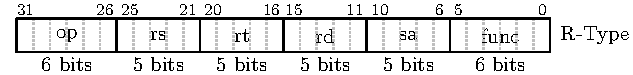
\includegraphics[scale=1.3]{MIPS_RType}
\caption{\ac{MIPS} \Rtype instruction encoding.}
\label{Figure:MIPS_RType_encoding}
\end{figure}
%

In \Rtype instructions, \code{op} field has a constant value of \code{6'b000000}. 
The actual operation to be performed in \Rtype instructions is given by the \code{func} field.
By contrast, for \Itype and \Jtype instructions, \code{op} presents different values and field \code{func} is not present.

% ======================================
% Specifications
% ======================================
\section{Design specifications}
The following sections provide an overview of the design specifications for this assignment.

\subsection{General specifications}\label{sec:general_specs}
Your custom \ac{MIPS} design must comply with the following design specifications.
%
\begin{itemize}
\item Instruction set based (but modified) on a standard 16-bit \ac{MIPS} \ac{uP}.
\item Single-cycle design.
\item Data width is 16-bits.
\item Instruction encoding (instruction width) is 32-bits long.
\item \ac{RF} contains 32 registers.
\begin{itemize}
\item \code{r0} \alertblue{must} always be 0, \ie, \code{r0} is not writeable.
\item \code{r31} is return address.
\end{itemize}
\end{itemize}
%

\newpage
\subsection{\Rtype datapath}
\fref{figure:RType_schematics} shows the instruction encoding and the \ac{uA} diagram required in order to perform an arithmetic/logic custom \ac{MIPS} \Rtype instruction.
%
\begin{figure}[!htb]
\centering
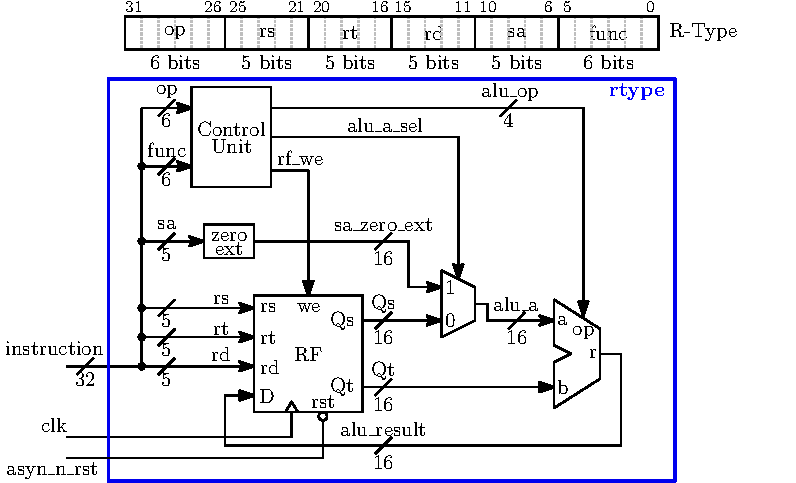
\includegraphics[width=\textwidth]{MIPS_design_Rtype_assignment}
\caption{\ac{MIPS} R-Type arithmetic/logic instruction partial datapath.}
\label{figure:RType_schematics}
\end{figure}
%

Here, the blue box in \fref{figure:RType_schematics} represents the top-level module, named \codeblue{rtype}.
\tref{table:toplevel_ports} specifies the top-level ports required for this assignment.
%
\begin{table}[!htb]
\centering
\caption{Top-level ports.}
\label{table:toplevel_ports}
\begin{tabular}{l|l|c|l}
\hline\hline
Port name & Direction & Width & Description \\
\hline\hline
\code{clk}          & \code{input} & 1 & Clock signal \\ \hline
\code{asyn\_n\_rst} & \code{input} & 1 & Asynchronous active-low reset \\ \hline
\code{instruction}  & \code{input} & 32 & Encoded instruction to be performed \\ \hline
 \end{tabular}
\end{table}
%

This top-level module consists of only three input ports, namely \clk, \asynnrst and \instruction, which correspond to the clock signal, an asynchronous active-low reset and the \Rtype instruction to be performed, respectively. 
Note that there are no output ports in this design since the result provided by the \ac{ALU} must be stored back into the \ac{RF}.



\newpage
\subsection{List of \Rtype instructions}
Your design must be able to perform the instructions specified in \tref{Table:MIPS_RType_examples}.

\begin{table}[htbp]
  \caption{\Rtype instructions.}
  \label{Table:MIPS_RType_examples}
  \centering
    \begin{tabular}{l|l|l}
    \hline\hline
    Instruction & Syntax & Meaning \\ \hline
    \code{ADD}  & \code{ADD rd, rs, rt}  & \code{rd $\leftarrow$ rs + rt}\\ \hline
    \code{SUB}  & \code{SUB rd, rs, rt}  & \code{rd $\leftarrow$ rs - rt}\\ \hline
    \code{NAND} & \code{NAND rd, rs, rt}  & \code{rd $\leftarrow$ $\sim$(rs \& rt)}\\ \hline
    \code{NOR}  & \code{NOR rd, rs, rt}  & \code{rd $\leftarrow$ $\sim$(rs | rt)}\\ \hline
    \code{XNOR} & \code{XNOR rd, rs, rt} & \code{rd $\leftarrow$ $\sim$(rs \^{} rt)}\\ \hline
    \code{AND}  & \code{AND rd, rs, rt}  & \code{rd $\leftarrow$ rs \& rt}\\ \hline
    \code{OR}   & \code{OR rd, rs, rt}   & \code{rd $\leftarrow$ rs | rt}\\ \hline
    \code{XOR}  & \code{XOR rd, rs, rt}  & \code{rd $\leftarrow$ rs \^{} rt}\\ \hline
    \code{SLL}  & \code{SLL rd, rs, sa} & \code{rd $\leftarrow$ rt $<<$ sa}\\ \hline
    \code{SRL}  & \code{SLL rd, rs, sa} & \code{rd $\leftarrow$ rt $>>$ sa}\\ \hline
    \code{SLA}  & \code{SLL rd, rs, sa} & \code{rd $\leftarrow$ rt $<<<$ sa}\\ \hline
    \code{SRA}  & \code{SLL rd, rs, sa} & \code{rd $\leftarrow$ rt $>>>$ sa}\\ \hline
    \hline
  \end{tabular}
\end{table}

\subsection{Description of each submodule}\label{sec:submodules}
The following sections provide a brief description about each of the submodules presented in \fref{figure:RType_schematics}.



\subsubsection{\acl{RF}}
The \ac{RF} of \fref{figure:RType_schematics} stores the contents of the 32 available registers.
As indicated in \sref{sec:general_specs}, \code{r0} must contain a constant value of 0. 
This implies that \code{r0} must not be writeable.
As a result of this, your \ac{RF} design must be updated in order to prevent write operations to be performed on \code{r0}.
All other registers, including \code{r31} which will be used in \Jtype instructions, may be written to.
Similarly, you may have to update your \code{rf} module in order to comply with the following input and output ports.
The inputs to this module are two source (read) registers \rs and \rt, a destination (write) register \rd, input data \aluresult provided by the \ac{ALU}, a control signal \rfwe provided by the control unit for write operations and a \clk and an asynchronous active-low reset \asynnrst.
This module provides at each clock cycle outputs \Qs and \Qt, which correspond to data stored in registers \rs and \rt, respectively. 
These outputs correspond to operands required by the \ac{ALU}.

\subsubsection{\acs{ALU}}
The \ac{ALU} of \fref{figure:RType_schematics} performs the arithmetic and logical operations specified by the \instruction.
More specifically, signal \aluop provided by the control unit determines which operation the \ac{ALU} must perform.
Input \signalname{a} of the \ac{ALU} is connected to signal \alua, which corresponds to either output \Qs from the \ac{RF} or a zero-extended version of the field \sa from \instruction. 
This is due to the fact that field \sa is used to determine the shift amount in shift-type operations in the \ac{ALU}.
However, since \sa is only 5-bits, it must first be zero-extended to 16 bits.
The selection of \alua is determined by the \ac{MUX} of \fref{figure:RType_schematics} and its control signal \aluasel provided by the control unit. 

\subsubsection{Control Unit}
The control unit of \fref{figure:RType_schematics} commands other submodules in the design.
This is performed by using several control signals, for example, enable signals.
The control unit of the \Rtype datapath instructs the \ac{RF} to write its coming data \aluresult from the \ac{ALU} by means of the \rfwe signal.
It also instructs the \ac{MUX} to provide to operand \signalname{a} of the \ac{ALU} either the zero-extended version of \sa or the output \Qs from the \ac{RF}.
This is achieved by means of \aluasel signal.
Finally, the control unit instructs the \ac{ALU} which of the 15 operations it must perform by means of the signal \aluop.
These control signal are asserted according the input signals \op and \func.
More specifically, since \Rtype instructions are defined with \op \code{= 6'b000000}, the actual \ac{ALU} operation will be determined by the value of \func.
A suggested mapping between \func and \aluop is provided in \tref{Table:func_ALU_mapping}.
\begin{table}[htbp]
  \caption{Suggested mapping between \code{func} and \code{alu\_op}.}
  \label{Table:func_ALU_mapping}
  \centering
    \begin{tabular}{l|l}
    \hline\hline
    \code{func} & \ac{ALU} operation  \\ \hline
    \code{6'b100000}  & \code{ADD}  \\ \hline
    \code{6'b100010}  & \code{SUB}  \\ \hline
    \code{6'b110100}  & \code{NAND}  \\ \hline
    \code{6'b110101}  & \code{NOR}  \\ \hline
    \code{6'b110110}  & \code{XNOR} \\ \hline
    \code{6'b100100}  & \code{AND}  \\ \hline
    \code{6'b100101}  & \code{OR}   \\ \hline
    \code{6'b100110}  & \code{XOR}  \\ \hline
    \code{6'b000000}  & \code{SLL} \\ \hline
    \code{6'b000010}  & \code{SRL} \\ \hline
    \code{6'b000001}  & \code{SLA} \\ \hline
    \code{6'b000011}  & \code{SRA} \\ \hline
    \hline
  \end{tabular}
\end{table}

Note that your \ac{ALU} design supports operations that are not listed in \tref{Table:func_ALU_mapping}. 
This is due to the fact that operations such as \code{LUI} and \code{LLI} are part of \Itype instructions.

As part of the requirements, you \alertred{must} use a \SV user-defined data type for defining all \func values.
The user-defined data type may be declared as in \lref{listing:func_t}
\lstset{numbers=none, xleftmargin=.1\textwidth, xrightmargin=.1\textwidth , caption={Definition of \code{func\_t} data type.},label=listing:func_t}
\begin{lstlisting}
typedef enum logic [5:0] { // Width and type of data type
  ADD_FUNC: 6'b100000,     // addition
  SUB_FUNC: 6'b100001,     // subtraction
  // all remaining func values
} func_t;                  // Name of data type
\end{lstlisting}

\newcommand{\mipspkgfile}{\colorfilename{mips\_pkg.sv}}
\subsection{\SV design files}\label{sec:SV_files}
The minimum required \SV design files are listed below.
You may decide to create new \SV modules and files in order to create different hierarchy levels. 
For example, you may decide to create a \SV module specifically for instruction decoding inside the control unit.
\begin{itemize}
\item \mipspkgfile. Package file common to all design files. 
You must declare all the necessary parameters and data types in this file.
\item \rtypefile. \Rtype top-level module. 
This module instantiates all the submodules such as \code{rf}, \code{alu}, \code{sgn\_ext}, \code{mux\_2x1}, and \code{control\_unit}.
The connections among the different submodules may be done using glue logic, \ie, signal assignments for interconnecting all submodules.
For example, the input port \instruction must divided into several signals for different submodules.
\item \rffile. \ac{RF} module description.
\item \alufile. \ac{ALU} module description.
\item \sgnextfile. Zero/sign extender module description.
\item \muxfile{2}. 2x1 \ac{MUX} module description.
\item \controlfile. Control unit module description.
\end{itemize}

% ======================================
% Grading criteria
% ====================================== 
\section{Grading criteria}\label{sec:Grading}
The following grading criteria will be considered.

\begin{enumerate}
\item \alertblue{The correct functionality of your designs.}
I will use my own testbenches in order to automatically stress your designs and verify that they perform the tasks according to the specifications. 
For example, I will try different values for the parameters in your designs and I expect them to still perform according to the specifications.
This is why it is paramount that you follow the name convention specified for file names and port names.
Moreover, it is important that your designs and testbenches compile in \ModelSim without errors.
\alertred{Your maximum grade for this assignment will automatically drop to 50/100 should \ModelSim trigger a compilation or simulation error.}
\item \alertblue{The quality of your testbenches.}
Even though I will use my own testbenches, I expect you to consider a thorough and concious set of test scenarios.
In this way, you should be able to spot any mismatches between the expected results and the actual results provided by your designs.
\item \alertblue{Your designs must be synthesized in \Quartus without latches and without errors.}
Warnings are tolerated at this point.
\alertred{Your maximum grade for this assignment will automatically drop to 50/100 should \Quartus trigger a synthesis error or generate unwanted latches.}
Remember that a design is not useful if it can't be synthesized.
\end{enumerate}


% ======================================
% Deliverables and Submission instructions
% ====================================== 
\section{Deliverables and Submission instructions}\label{sec:Deliverables}
Prepare a single \code{zip} file containing \alertred{at least} the following files.
You may have created additional \SV modules as stated in \sref{sec:SV_files}.
If that's the case, please include them in your \code{zip} file.
\begin{enumerate}
\item \mipspkgfile.
\item \rtypefile.
\item \rtypetbfile. Testbench for your top-level \Rtype design.
\item \rffile.
\item \alufile.
\item \sgnextfile.
\item \muxfile{2}.
\item \controlfile.
\item \rtypedofile. \ModelSim script for compiling and simulating your design. You may decide to breakdown your \ModelSim script into several scripts for separating each design step.
\item A \Quartus \ac{RTL} screenshot of your synthesized top-level \Rtype design.
\end{enumerate}

Submit your assignment through Canvas \alertred{no later} than \deadline.
\\
Please send any questions to \href{mailto:isaac.perez.andrade@tec.mx}{isaac.perez.andrade@tec.mx}.
\end{document}
